\section{Tidal circularization}
%
\label{sec:synchronization_circularization_alignment}

The effect of tides scales as the difference in the gravitational acceleration
due to the companion at the near and far tidal bulges multiplied by the mass in
each bulge. Both of these factors themselves are a strong function of the ratio
of the size of the object to the size of the orbit. As a result, the tidal
coupling between a planet and its host star decreases very rapidly as the
distance between the planet and the star increases. This is why tides are only
important for planets which get very close to their parent stars at least for
some part of their orbit.

As described in the previous section, planetary tides exchange angular
momentum between the orbit and spin of the planet, stellar tides exchange
angular momentum between the orbit and spin of the star, and both tides extract
energy out of the system, leading to orbital circularization.

The quantity that is most readily affected by tides is the spin of the planet.
This is due to two reasons. First, the angular momentum of the planet is many
orders of magnitude smaller than both the orbital and stellar angular momenta,
so it most easily affect. Second, the self-gravity of the planet is much smaller
than that of the star, and the tidal force on the planet is much larger than
that on the star. Since the size of the tidal bulges is determined by the
competition between self-gravity and tidal force, the planetary tides are much
stronger. As a consequence, the expectation is that pseudo-synchronizing the
planet's spin with the orbit should be the tidal signature affecting the largest
number of exoplanet systems. Unfortunately, at present, there is no way to
observationally determine the spin of an exoplanet, so we cannot test this
prediction.

\begin{figure}[t]
%
    \centering
%
    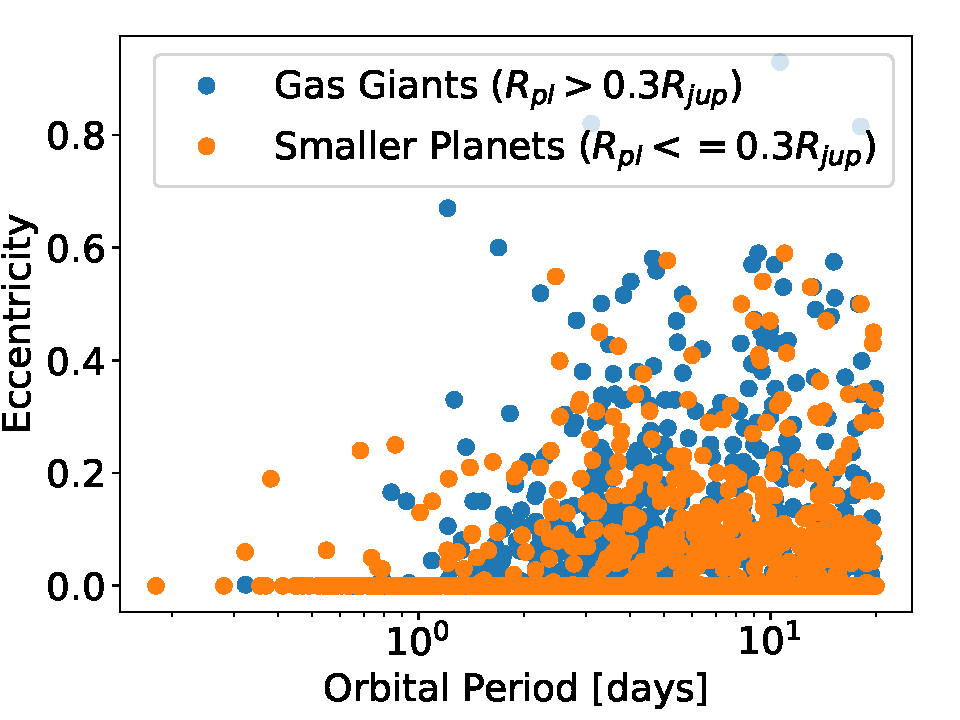
\includegraphics[width=0.5\textwidth]{period_eccentricity.pdf}
%
    \caption{
%
        The period vs eccentricity of the currently confirm extrasolar planets
        from the NASA exoplanet archive. The color indicates the radius of the
        planet.
%
    }
%
    \label{fig:period-eccentricity}
%
\end{figure}

The second most strongly tidally affected property of exoplanet systems is the
eccentricity of their orbits. For most systems the orbital angular momentum is
smaller than the stellar spin angular momentum and it is feeling the combined
effect of both stellar and planetary tides, with the latter being significantly
more important as long as the eccentricity is not negligible. The observational
evidence of tides on the orbital eccentricity is that the shorted period
systems, which experience the strongest tides, get circularized very quickly, so
they are all observed in circular orbits, with gradually more and more
eccentricity surviving at longer and longer orbital periods (see
Fig.~\ref{fig:period-eccentricity}).

There is an important difference between circularization due to stellar vs.\
planetary tides. Each type of tide couples the orbit to the spin of the
corresponding object. Since the planet's spin angular momentum is negligible
compared to the orbital angular momentum, to an excellent approximation,
planetary tides cannot change the orbital angular momentum. This can be shown to
imply that if only planetary tides are present, circularization will proceed in
such a way as to hold $r_p(1+e)$ constant, where $r_p$ is the so called
pericenter distance (the distance of closest approach between the planet and the
star) and $e$ is the eccentricity. In other words, under only planetary tides,
circularization is inevitably accompanied by an increase in the distance of
closest approach between the star and the planet. Since tides are strongest at
pericenter, this generally decreases the rate of circularization over time.

This is in contrast to the case of stellar tides, where the stellar spin angular
momentum is comparable to or perhaps even dominates over the orbital angular
momentum. In this case, the pericenter distance can grow or shrink, depending on
the stellar spin and orbital configuration. Sun-like stars in particular have
spin periods longer than a few days for most of their main-sequence lifetime.
Since tidal circularization is only important for orbital periods of a few days
or less, stellar tides will mostly decrease the angular momentum of the orbit
over time, resulting in smaller pericenter distance compared to planetary
tides.

\section{Tidal inspiral}

Another effect that is expected to occur in very short period exoplanet systems
is tidal inspiral. This is only relevant for exoplanet systems whose orbital
period is short enough for the tides on the planet to have circularized the
orbit and synchronized the spin of the planet with it. As a result, the
planetary tides are now static on the surface of the planet and no longer
experience friction. This leaves only stellar tides to drive further evolution.
Stars generally have spin periods exceeding the orbital period. As discussed
above, this situation leads to tidal bulges that lag behind the planet as it
move around in its orbit, leading to removal of angular momentum from the orbit
and adding it to the spin of the star. Since stars have hundreds to thousands of
times more mass than even the most massive planets, their moment of inertia is
in almost all cases large enough to prevent the star from synchronizing to the
orbital period of the planet. As a result, stellar tides gradually shrink the
orbit of the planet, driving it closer and closer to the star.

If the planet starts out relatively far away from the star, this inspiral could
take longer than the lifetime of the star, but for the shortest period systems,
this will eventually push the planet close enough to its parent star for one of
two things to happen. First, tides get stronger as the planet-star separation
decreases, until the tidal force attempting to stretch the planet overwhelms the
self-gravity of the planet. This will cause the planet to be tidally ripped
apart. The distance between the planet and the star at which this occurs is
known as the Roche limit, and it depends on the size and mass of the planet. The
more massive the planet is, the stronger its self gravity, pushing the Roche
limit closer to the star.  Similarly, the larger the planet, the weaker its self
gravity, and hence the Roche limit is pushed further away. In the case of gas
giant planets, the Roche limit is comparable to the size of the star. For some
planets, it lies inside the star, in which case the planet will be engulfed by
the star still relatively intact. In either case, the tidal inspiral will cause
the destruction of the planet.

Currently, a number of researchers have claimed to directly detect shortening of
the orbital periods of exoplanets over time by observing a shortening of the
time between consecutive transits. For example, the very firs planet discovered
by the \textit{Kepler} space satellite Kepler-1658 (a.k.a KOI-4) appears to be
shrinking \citep{Vissapragada_et_al_22}. \citet{Maciejewski_et_al_16} also claim
to detect orbital decay in the system WASP-12. This finding was independently
confirmed by \citet{Patra_et_al_17}. At the moment it is hard to rule out
alternative explanations for the observed it is hard to be completely certain
that what is observed is indeed orbital decay as opposed to for example orbital
precession or the effect of undetected third bodies in these exoplanet systems.
Furthermore, even if the orbits of these planets are indeed decaying,
unequivocally attributing that decay with tidal dissipation in the star is far
from straightforward.

Two separate lines of evidence point to this process occurring for gas giant
exoplanets, while perhaps not for smaller, rocky planets. First,
\citet{Jackson_et_al_09} pointed out that the smallest orbits in which younger
exoplanet systems are observed are smaller than the smallest orbits in which
older systems are observed. This is matches the predictions of the tidal
inspiral scenario, as the older systems have more time to be affected by tides
and hence systems beginning with larger separations will inspiral and be
destroyed. A different line of evidence for the tidal destruction of the
shortest orbital period exoplanets comes from their velocities within the
galaxy. \citet{Hamer_Schlaufman_19} compared the host stars of giant planets in
orbits with periods few days (a.k.a. hot Jupiters) to two control samples of
stars without planets, and stars with longer period planets. What they found is
that the velocities of hot Jupiter hosts show much smaller scatter around the
mean rotation of the galaxy less than either of the control samples, while the
distribution of velocities of the two control samples are statistically
indistinguishable. It is a well established property of our galaxy that the
smaller the scatter in the velocities of a sample of stars, the younger it is.
Hence, this observation is another indication of the relative youth of systems
containing short period giant planets, suggesting the older systems have lost
their planets to tidal inspiral.

\section{Tidal spin-up of Sun-like exoplanet host stars}

Sun-like stars gradually spin down over time. This spin-down is faster the
faster the star spins, which causes the spin periods of these stars to converge
over time. As a result, isolated Sun-like stars older than a few hundred million
years have a spin period tightly related to their age. Measuring the rotation
and using this relationship is one of very few methods of determining the ages
of isolated stars.

For stars experiencing tides however, this unique spin-age relationship can be
broken. For exoplanets experiencing tidal inspiral the host star is expected to
spin faster than an isolated star of the same age would. This is direct
consequence of angular momentum conservation. As tides drive the planet closer
to its parent star, the orbital angular momentum that is lost gets added to the
stellar spin. One would expect then that stars with short period giant
exoplanets orbiting them will spin on average faster than similar isolated stars
or stars with longer period or small planets. In fact, \citet{Tajeda_et_al_21}
claims to confirm this prediction.

On the one hand, this is unfortunate, since measuring the rotation period of
stars and using the spin-age relationship is one of very few ways of determining
stellar ages. The fact that tides affect the spin, means this method can not be
reliably used for hot Jupiter hosts. On the other hand, \citet{Penev_et_al_18}
suggest that the deviation from single star spin evolution is significant enough
to be used as a probe of the tidal dissipation physics of Sun-like stars. The
latter is particularly important as exoplanet systems are sensitive to a
different regime of tides than binary stars. Only stellar tides affect the
stellar spin, unlike the effects on the orbit, for which as long as eccentricity
is non-zero, both stellar and the planetary tides are important.

\section{Tidal alignment}

The tidal torque due to the stellar tides on the orbit will also cause the orbit
to align with the equator of the star. This is one of the leading explanations
for the observed trend that giant planets orbiting Sun-like stars appear to
have orbits that are aligned with the stellar equator, while stars significantly
more massive, and hence hotter, than the sun, seem to host planets with all
kinds of orbital orientations \citep[c.f. chapter 5.2 of][]{Winn_Fabrycky_2015}.
The lack of alignment between hot stars and the orbits of their companion
planets has been hypothesized to be due to much weaker tidal friction that is
expected to occur in these stars. More specifically, the transition between
aligned and misaligned orbits appears to coincide with the transition between
stars that have surface convective zones and those that do not, and the
turbulent flow present in stellar convective zones has long been thought to be
one of the leading causes of tidal friction.

It must be emphasized, however, that the tidal interpretation of the observed
alignment pattern is far from universally accepted.  Alternative suggestions
include the possibility that most planets generally form aligned, with various
mechanisms causing misalignment in some systems. That said, the tidal
explanation is one of the most compelling, since it does not require assuming
any new physics.

In general, all proposed explanations for the observed alignment pattern,
including the tidal one, have at least one significant problem they need to
overcome. In the case of tides, the issue is one of timescales. As we discussed
in the introduction, the timescale for tidal inspiral is comparable to or
shorter than the timescale on which the stellar spin is affected by tides. As a
result, any system which has been appreciably tidally aligned, should also have
experienced significant inspiral. As all tidal timescales decrease very
dramatically as the orbit gets smaller, this in turn implies that the planet has
only a short time remaining to live before tides drive it into the star. This is
statistically implausible. While detecting shorter period planets is somewhat
easier than longer period ones, the difference is not large enough to match what
would be naively predicted if tides are responsible for the observed alignment
pattern. This problem could be resolved by more realistic tidal dissipation
theories than the somewhat simplistic treatment discussed in the introduction
(see \citep{Lai_12} and \citep{Anderson_et_al_21}).

\section{Tidally heating and inflating exoplanets}

Tidal friction converts some of the mechanical energy of tidal deformations into
heat. This heating is irrelevant for the star, since it only constitutes a
negligible fraction of the stellar luminosity. However, for the planet this may
not be the case.

In our own solar system we have several rather dramatic examples where
tidal heating drives spectacular geological processes. For example, the tidal
heating of Saturn's moon Enceladus is thought to be responsible for powering
spectacular eruptions of water icy particles and gas from the moon's south pole.
The best to-date accounting for the energy budget of Enceladus suggests that
this geologically active region on Enceladus accounts for roughly a quarter of
the entire energy budget of that moon, even though it covers less than 5\% of
the surface.

In the case of exoplanets, we do not yet have any firm direct evidence of the
importance of tidal heating, but it has been speculated to be an important
mechanism affecting the sizes of hot Jupiters. Many hot Jupiters are observed to
have sizes that are larger than can be explained by standard models of planetary
structure, and one of the proposed explanations for these inflated radii is
tidal heating.

Even though the energy delivered by tidal dissipation may be small compared to
direct irradiation by the star, it can have an outsized impact. Because, even
though stellar irradiation deposits massive amounts of energy, it does so at
optical depths of order unity, where it is quickly radiated away without
significantly affecting the internal structure of the planet. In contrast,
\citet{Komacek_Youdin_17} argue that even orders of magnitude smaller heating,
if deposited deeper into the planet can have a profound effect on the planetary
radius.

In order for tides to heat, and as a result, inflate a planet, the planet needs
to either be in an orbit with non-zero eccentricity, or have a spin period that
is not exactly equal to its orbital period. For planets spinning synchronously
in circular orbits the tidal deformation is static, and no energy is dissipated.
This can be a temporary situation the lifetime of a planet, if it begins in a
significantly eccentric orbit, or if its orbital eccentricity is somehow excited
(e.g. by gravitational interactions with other planets in the system). Such
situations will typically occur early in the life of an exoplanet system. In
fact, excitation of the eccentricity to very large values, followed by tidal
circularization is one of the mechanisms proposed for how some of the shorter
period exoplanets come to be in their current orbits. However, by the time the
host stars reach the main sequence, such processes will mostly have played out,
leaving planets experiencing strong tides in circular orbits with their spins
synchronized to the orbital period.

One mechanism that can prevent tidal circularization is the presence of
additional planets in the system. Since our planet detection methods are not
100\% effective, even if no additional planets are observed they may be there.
Particularly important are planets residing close to mean motion resonances as
described in Section \ref{sec:equilibrium}. In the case of Enceladus mentioned
above, the orbit is observed to be slightly eccentric. Its orbital eccentricity
is maintained by interactions with one of the other moons of Saturn: Dione,
which is in a 2:1 mean motion resonance with Enceladus.

Alternatively, or perhaps in addition, it is possible that some mechanism
counteracts tidal synchronization, again maintaining some degree of asynchrony.
One such proposed mechanism are the so-called thermal (or atmospheric) tides.
Very briefly, thermal tides refers to fluid motions in the atmosphere of the
planet that are driven by time-variable stellar irradiation. Variable
irradiation can arise because of orbital eccentricity, tilt of the planet's axis
of rotation relative to the orbital plane (e.g. the seasons on Earth), or
because of asynchronous rotation. The fluid mechanical response to such variable
heating of the atmosphere is in general quite a complicated process that is
outside the scope of this introductory chapter, but the ultimate result is that
the resulting redistribution of mass can alter the tidal potential of the planet
in addition to the effects of its tidal distortion. In turn this modified tidal
potential results in the equilibrium eccentricity of the orbit being non-zero
and/or the equilibrium spin of the planet to not be precisely synchronous. If
these departures from synchrony and circularity are large enough, tidal
dissipation within the planet can produce significant heat, possibly inflating
the planet, and accelerating its orbital decay beyond what the tidal dissipation
within the star alone can provide. \citet{Arras_Socrates_10} argue that at
least in principle, this effect could provide sufficient heating to explain the
observed radius inflation of hot Jupiters.
